
%(BEGIN_QUESTION)
% Copyright 2010, Tony R. Kuphaldt, released under the Creative Commons Attribution License (v 1.0)
% This means you may do almost anything with this work of mine, so long as you give me proper credit

Using a PLC with at least two switches pre-wired to its input terminals and an HMI panel connected to a communications port, write a ladder-logic program to control the operation of a motor.  If your PLC's switches are toggle rather than pushbutton, you may simulate the momentary contact of a pushbutton by ``flicking'' the toggle switch back and forth.  No devices need be wired to the PLC's output terminals:

$$\includegraphics[width=15.5cm]{i02441x01.eps}$$

\noindent
The basic idea of this control system is to give a human operator the ability to do the following:

\vskip 10pt

\begin{itemize}
\item{} \underbar{Start} and \underbar{Stop} the motor from hard-wired switch controls
\vskip 10pt
\item{} \underbar{Start} and \underbar{Stop} the motor from HMI controls
\vskip 10pt
\item{} \underbar{Count} and \underbar{display} how many times the motor has started
\vskip 10pt
\item{} \underbar{Time} and \underbar{display} the total number of seconds the motor has run (accumulative)
\vskip 10pt
\item{} \underbar{Calculate} and \underbar{display} some parameter of the motor's run history
\end{itemize}

\vskip 10pt

\noindent
Points shall be awarded for the successful demonstration of these and other functions.  

\vfil \eject

\hrule
\vskip 10pt

\noindent
{\bf 10\% -- ``Start'' and ``Stop'' pushbutton functions}

When momentarily pressed, the ``Start'' pushbutton shall cause the motor to start and continue to run after releasing the switch.  This pushbutton switch shall be normally open (NO), which means it energizes its respective PLC input when pressed, and de-energizes its input when released.

When momentarily pressed, the ``Stop'' pushbutton shall cause the motor to ``unlatch'' from its running condition.  If both ``Start'' and ``Stop'' pushbuttons are simultaneously pressed, the motor shall stop.  This pushbutton switch shall be normally closed (NC), which means it de-energizes its respective PLC input when pressed, and energizes its input when released.

\vskip 10pt
\hrule
\vskip 10pt

\noindent
{\bf 10\% -- ``Start'' and ``Stop'' HMI pushbutton functions}

When momentarily pressed, a ``Start'' control on the HMI shall cause the motor to start and continue to run after releasing the switch.  This ``pushbutton'' shall be momentary in operation, not latching or toggling.

When momentarily pressed, a ``Stop'' control on the HMI shall cause the motor to ``unlatch'' from its running condition.  This ``pushbutton'' shall be momentary in operation, not latching or toggling.

\vskip 10pt
\hrule
\vskip 10pt

\noindent
{\bf 10\% -- Motor start counter}

The PLC shall count the number of times the motor starts up, and the HMI will display this number.  A ``pushbutton'' control on the HMI screen will reset this counter to zero when momentarily pressed.

\vskip 10pt
\hrule
\vskip 10pt

\noindent
{\bf 10\% -- Motor total run timer}

The PLC shall track the total accumulated run-time of the motor, in seconds, and the HMI will display this value on the screen.  This means the sum total of all run periods, regardless of how many times the motor has started and stopped.  A ``pushbutton'' control on the HMI screen will reset this timer to zero when momentarily pressed.

\vskip 10pt
\hrule
\vskip 10pt

\noindent
{\bf 10\% -- Average run time calculation}

The PLC will calculate the average run-time per start of the motor, and the HMI will display this value on the screen.  For example, if the motor was run once for 10 seconds (then shut off), then run once again for 20 seconds (then shut off), the HMI should display an average run time of 15 seconds per start.  If the motor is run once again for 30 seconds, the HMI's average run time per start should display 20 seconds per start.  This calculated value should continuously update as the motor runs.

\vfil \eject

\underbar{file i02441}
%(END_QUESTION)





%(BEGIN_ANSWER)


%(END_ANSWER)





%(BEGIN_NOTES)

{\bf This question is intended for exams only and not worksheets!}.

%(END_NOTES)

